\documentclass[12pt]{article}

\usepackage[utf8]{inputenc}
\usepackage{sfmath}
\usepackage{amsmath}
\usepackage{graphics}
\usepackage{graphicx}
\usepackage{subfig}
\usepackage{wrapfig}
\usepackage{lipsum}

\usepackage[super, sort&compress]{natbib}
\usepackage{hyperref}
\usepackage{url}

\usepackage{tikz}
\usetikzlibrary{shapes.geometric}
 
\usepackage{physics}

\usepackage{titling}
\pretitle{\begin{center}\Huge\bfseries}
\posttitle{\par\end{center}\vspace{0.5cm}}
\preauthor{\begin{center}\large}
\postauthor{\par\end{center}}
\predate{\begin{center}\large}
\postdate{\par\end{center}}

\usepackage{geometry}
\geometry{a4paper, margin=1in}

\title{
    Mechatronics and Making \\
    Mid-Term Project Report \\
    Exoskeleton Robotic Hand With Wolf Claw Mechanism
}


\author{
    \begin{align*}
        \text{Bryan Li}\ &-  \text{SN 25003743} \\
        \text{Yan Pei Zhu}\ &-  \text{SN 25103352}\\
        \text{Nolan Yu}\ &-  \text{SN 25113715}
    \end{align*}
}

\date{October 31, 2025}

\setlength{\parindent}{0pt}
\setlength{\parskip}{1em}


\begin{document}

\begin{titlepage}
	\maketitle
\end{titlepage}

\tableofcontents

\pagebreak



\section{Project Objectives and Description}	%% ============================ SECTION I ===================================

We examined the percentage of people who were victims of stalking in the last year, 
with 19.9\% of women since the age of 16 suffering from this abuse, 
of which 8.05\% were single women~\cite{ons_stalking_2025}. 
This data highlights the significance of our mechanism, 
as it increases the safety of the victim when physically approached by the stalker. 
However, this mechanism would be considered a weapon with the intention of using 
it for self-defence, which violates the Criminal Justice and Immigration Act 2008\cite{CriminalJustice2008}. 
Hence, to legalise our mechanism, we modified the dangerous component (the three wolf claws) 
into a blunt claw-shaped design made of PLA materials. With the aim of this mechanism serving 
as a cosplay prop and the objective of helping with self-defence- the self-defence aspect will 
be further examined in section 2.3, wolf claw mechanism comparison. 

\subsection{Similar Mechanisms}

There are many applications of exoskeleton robotic hands in 
diverse fields (e.g.\ rehabilitation medicine) in which most 
of these exoskeleton hands are powered. Our mechanism is purely 
passive as it allows a lightweight approach and only relies on 
the user's instinctive movements. Powered exoskeleton robotic 
hands tend to have higher demands regarding control schemes 
and mechanical design (involving actuators).  

The robotic hand should have the same DOFs as a human, yet 
given the compact size of the hand, it becomes impractical to 
actively control every joint~\cite{rosen2019wearableC8} when the complexity of the control 
algorithms increases with the DOFs in a powered exoskeleton 
robotic hand. 
Thus, some motions are left passive (passive DOF), 
power and control signals of the hand must also be 
routed such that it does not interfere with motion of 
arm, where we will be placing the wolf claw mechanism. 
Taking the increased mass and inertia into consideration, 
we have decided to design our mechanism in a purely mechanical 
way since there is no reliance on power source and is less 
susceptible to technical malfunctions.

A 1 DOF kinematic architecture~\cite{rosen2019wearableC9} has been used for the DIP 
(distal Interphalangeal joint) and PIP (proximal Interphalangeal joint) 
as it allows precise replication of the natural grasping motion.

\subsection{Industrial Applications} 

The exoskeleton robotic hand of our mechanism is purely passive, 
providing support for the fingers and hand during tasks that require 
a sustained grip on tools for long periods. By redistributing the physical 
load from the fingers to the palm exoskeleton (connected to the wrist and arm) 
and supporting proper posture, the user is less likely to suffer from overuse injuries. 
This mechanism could be used for repetitive tasks, such as manual labour in construction, 
or it could be used in further designing or developing powered exoskeleton hands.

\pagebreak

\section{Mechanical and Mechanism Analysis}     %% ============================ SECTION II ==================================

\subsection{Drive Method and Transmission}
This robotic hand exoskeleton uses an acceleration-based machinery system, 
amplifying the movements of the finger. 

This is achieved using a planetary gear mechanism connected to a string 
transmission and a pulley and belt system.

Details of the transmission process shown below:

\begin{center}
	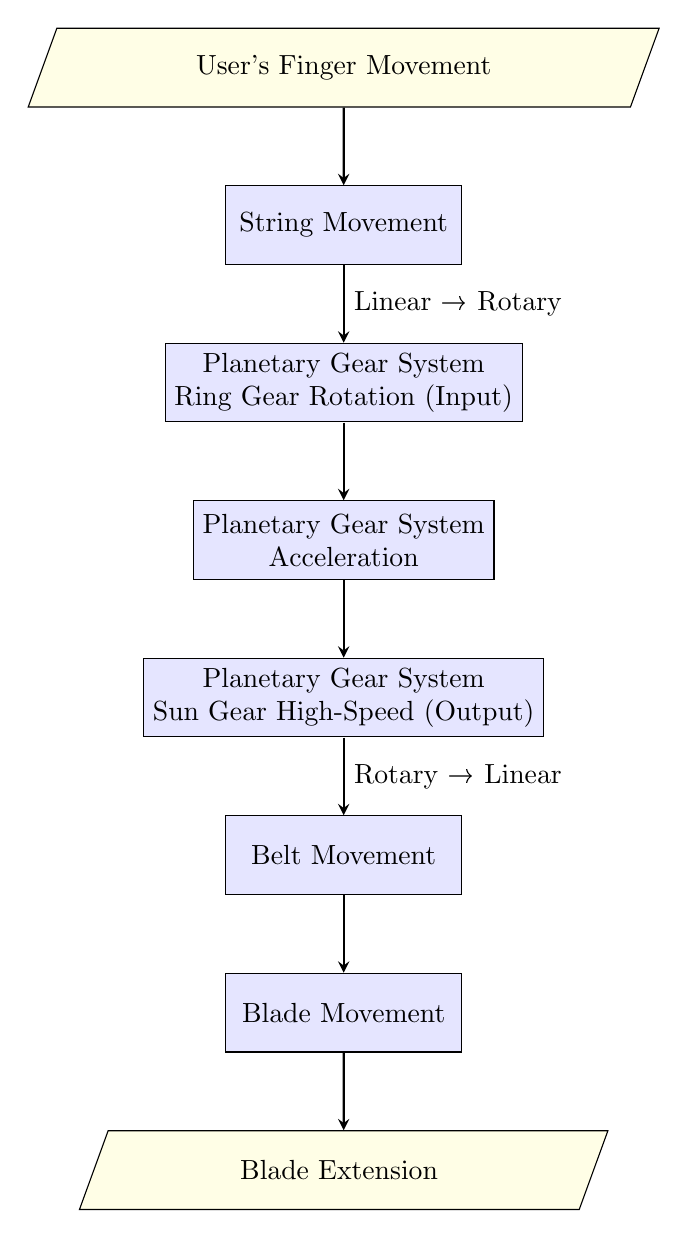
\begin{tikzpicture}[scale=0.8]

		% Define styles
		\tikzstyle{process} = [
		rectangle, minimum width=3cm, minimum height=1cm,
		text centered, draw=black, fill=blue!10, align=center]
		\tikzstyle{io} = [
		trapezium, trapezium left angle=70,
		trapezium right angle=110, minimum width=3cm,
		minimum height=1cm, text centered, draw=black,
		fill=yellow!10, align=center]
		\tikzstyle{arrow} = [thick,->,>=stealth]

		% Nodes
		\node (start) [io] {User's Finger Movement};

		\node (tendon) [process, below of=start, yshift=-1cm] {String Movement};

		\node (ring) [process, below of=tendon, yshift=-1cm] {
			Planetary Gear System \\
			Ring Gear Rotation (Input)
		};

		\node (planetary) [process, below of=ring, yshift=-1cm] {
			Planetary Gear System \\
			Acceleration
		};

		\node (sun) [process, below of=planetary, yshift=-1cm] {
			Planetary Gear System \\
			Sun Gear High-Speed (Output)
		};

		\node (pulley) [process, below of=sun, yshift=-1cm] {Belt Movement};

		\node (belt) [process, below of=pulley, yshift=-1cm] {Blade Movement};

		\node (blade) [io, below of=belt, yshift=-1cm] {
			Blade Extension
		};


		% Arrows
		\draw [arrow] (start) -- (tendon);
		\draw [arrow] (tendon) -- node[right] {Linear → Rotary} (ring);
		\draw [arrow] (ring) -- (planetary);
		\draw [arrow] (planetary) -- (sun);
		\draw [arrow] (sun) -- node[right] {Rotary → Linear}(pulley);
		\draw [arrow] (pulley) -- (belt);
		\draw [arrow] (belt) -- (blade);
	\end{tikzpicture}
\end{center}

\pagebreak

\subsection{Hand Exoskeleton Mechanisms Comparison}

\subsubsection{Hand Biomechanics}
Most human hands have 19 bones and 14~\cite{ons_stalking_2025} joints\cite{heo2012current}, excluding the carpal bones.

The design of the hand exoskeleton needs to be based on the natural anatomy of the 
human hand~(figure~\ref{fig:hand_label}). We have to focus on MCP, PIP, and 
DIP joints, because they ensure the finger can flex and extend easily.

\begin{figure}[htbp]
	\centering
	\subfloat[bones and joints of a human hand\cite{heo2012current}\label{fig:hand_skeleton}]{
		\includegraphics[width=0.45\textwidth]{imgs/bones_joints_of_hand.png}
	}
	\hfill
	\subfloat[model of human hand\cite{rosen2019wearableC8}\label{fig:hand_model}]{
		\includegraphics[width=0.45\textwidth]{imgs/model_of_the_hand.png}
	}
	\caption{Human Hand}\label{fig:hand_label}
\end{figure}

The finger joints include 3 types of joints majorly\cite{rosen2019wearableC8}:

Metacarpophalangeal Joint (MCP): \\
Has 2 degrees of freedom (flexion/extension, abduction/adduction).

Proximal Interphalangeal Joint (PIP): \\
Has 1 degree of freedom (flexion/extension).

Distal Interphalangeal Joint (DIP): \\
Has 1 degree of freedom (flexion/extension).

In the resting posture, the angle of MCP joint is approximately 45°, 
whereas the PIP joint is between 30°--45°, and the DIP joint is between 10°--20°.~\cite{heo2012current}
To define the range of motion and ensure safety in exoskeleton design, 
it is essential to align our mechanism to the human anatomy. 

\textbf{Wrist Structure Analysis}

The wrist has 2 degrees of freedom: flexion/extension and radial/ulnar deviation. 

\subsubsection{Selection of Mechanism Type}


Among the mechanisms illustrated in 
Figure~\ref{fig:mechanism_types}, the direct matching of joint 
centers (Figure~\ref{fig:mechanism_types}.a) was 
selected for our design because it provides a  
simple and compact solution without requiring additional 
linkages or complex actuation. 
Also, this approach minimises the mechanical complexity, 
reduces system weight, and simplifies both fabrication and control.

\begin{figure}[htbp]
    \centering
    \includegraphics[width=0.88\textwidth]{imgs/mechanism_types.png}
    \caption{mechanism types\cite{heo2012current}}\label{fig:mechanism_types}
\end{figure}

The exoskeleton joints directly aligned with 
the anatomical centers, which ensures high 
accuracy and reliability. This is because 
no additional compensation for motion is necessary. 

Therefore, the direct joint-center matching method offers the most 
efficient and practical solution for this application. 
We have chosen to take a similar approach

\pagebreak

\subsection{Wolf Claw Mechanism}
\textbf{Design of wolf claw}

Consider a wolf claw made of multiple sections:  

\begin{figure}[htbp]
    \centering
    \includegraphics[width=0.95\textwidth]{imgs/belt_and_claw.PNG}
    \caption{wolf claw blade movements section}\label{fig:wolf_belt_claw}
\end{figure}

\begin{figure}[htbp]
    \centering
    \includegraphics[width=0.70\textwidth]{imgs/blade3.PNG}
    \caption{3 blades}\label{fig:blade3}
\end{figure}

For this prototype the whole mechanism would be more portable due to these retractable features. 
For these retractable features to be implemented, the inner structure of each section of the wolf 
claw would be hollow, with only the tip of the claw being solid.  

The main challenges in this include how each section is going to connect as the number of 
sections increase, thus each section becomes thinner and the room for connection between 
adjacent links being reduced. When this wolf claw is extended, it becomes difficult to 
ensure the same section of each wolf claw extends simultaneously, smoothly and securely. 
As a consequence of not having any supports in the wolf claw, there will be oscillations 
in each section, with the tip of the wolf claw oscillating the most. Reflecting on the objective 
of this mechanism, this prototype is ineffectual as the structure of this wolf claw 
would lead to the sections easily snapping. 

Hence, we propose a different method, where each wolf claw is modelled as individual 
blades as it would still fulfil the intended purpose and objective. 
However, this approach would lead to the box containing the wolf claw mechanism being longer, 
problems that arise from this include how this box is going to be stabilised to the arm as it 
would be longer than a forearm of the average human.  

The three blades (Figure~\ref{fig:blade3}) are connected by a square bar along the top of the blades, 
perpendicular in the direction of the blades. These blades are not sharpened 
as the purpose is to act as a cosplay prop but to fulfil the objective effectively, 
these blades would have a sandpaper coating and be non-backdrivable. To allow this 
non-backdrivable feature, a spring plunger is integrated at the side of the box, 
locking the two side blades in position. In this mechanism we aim to make to make 
the wolf claw retract semi-automatically, hence we modified the spring plungers 
(see figure~\ref{fig:wolf_belt_claw}) so that they can retract by applying force to the handle. 

\textbf{Transmission Mechanism Selection}

The key feature of our design is sliding the wolf claws out, this achieved using a 
combination of planetary gears as part as a simple gear train. Another approach for 
the this would be using the structure of a compound gear train, let the two versions 
be versions one and two respectively. Both methods start with rotary-to-rotary motion, 
this is then converted from rotary to translational motion through the use of pulley and belt systems.  

\textbf{Version I:\ Planetary Gear}

This version provides a higher gear ratio with a 
more compact and stable design but requires high precision in 
laser cutting and 3D printing as several components mesh into the same gear.  

\textbf{Version II:\ Compound Gear Train}

This version is simpler to print and has a higher 
flexibility in gear ratios, yet there is a lack of stability in the 
blades as the centre blade drives the two side blades. 

Therefore, we would use version 1 for our first prototype.

\subsubsection{Version I:\ Planetary Gear}

The light inextensible string would be connected to the ring gear of 
the fixed carrier planetary gear. Both the fixed carrier gear and the 
sun gear would be extended to a height 
of $7$~mm, the fixed carrier gear would be 
fixed to the inside of top of the box. 
The sun gear will rotate together with another gear and mesh with 
gears A1 and B1 (shown Figure~\ref{fig:wolf_belt_claw}), 
which are identical and are fixed to the bottom of the box by screws.
This forms a simple 
gear train, further increasing the overall gear ratio. 

At the other end of the box, identical gears to A1 and B1 are fixed to the floor parallel 
to gears A1 and B1, let us call them A2 and B2. By using timing belts 
(shown in Figure~\ref{fig:wolf_belt_claw}), 
two pulleys and belts systems are formed between gears A1,2 and B1,2, allowing a higher 
efficiency with no slippage whilst dampening noise. Challenges in this design being the 
timing belts being difficult to put together as the timing belts are required to be flexible 
for our design.  When 3D printing each section of the timing belts, removing the supports 
was an arduous task with low success rates, hence we adapted the gears A1,2 and B1,2  
as shown in figure~\ref{fig:wolf_belt_claw} to use the open timing belts and timing pulleys in the 
innovation lab. The top section will allow the gears A1 and B1 to mesh properly with 
the sun gear, the bottom half would be glued into the timing pulley, meaning that 
gears A2 and B2 would just be a timing pulley with a fixed rod through the centre, 
fixed to the bottom of the box.  

\begin{figure}[htbp]
    \centering
    \includegraphics[width=0.70\textwidth]{imgs/planetray_vel.png}
    \caption{Linear velocity of input and blade out}\label{fig:planetray_vel}
\end{figure}

The two side blades would be fixed to these pulley and belt systems (A1,2 and B1,2) using 
superglue on the end of the blade, with a centre blade connected to a third pulley and belt 
system as shown in figure~\ref{fig:wolf_belt_claw}. The blades are connected to ensure all three blades slide out 
simultaneously, and stability of the centre blade can be increased by integrating a third pulley 
and belt system. This allows the motion of the centre blade to be parallel to the side blades 
when the whole mechanism is moving or when there is a force applied to the tip of the blades. 
When there is force applied on the blades, it may be impractical to hold the blades to the belt 
only by superglue at the end section of the blade, hence screwing the blades to the belt would 
make this mechanism more secure. Ensuring the open timing belts are tight would be challenging 
as the glue requires some time to dry and the timing belts must be held together tightly during 
this time, the difficulty in this being that it must align perfectly with the other end to ensure 
perfectly horizontal motion of blades.  


\pagebreak

\subsubsection{Version II:\ Compound Gear Train}
The compound gear train (Figure~\ref{fig:gear_comp}) is dependent on the contact between gears, reflecting on the objective 
of our mechanism, it is essential to ensure the gears mesh regardless of motion of mechanism.  

\begin{figure}[htbp]
	\centering
	\subfloat[compound gear train\label{fig:gear_comp}]{
		\includegraphics[width=0.45\textwidth]{imgs/gear_box_comp.PNG}
	}
	\hfill
	\subfloat[compound gears, pulley and belt system\label{fig:gear_comp_mech}]{
		\includegraphics[width=0.45\textwidth]{imgs/Compound-Gear-and-mech.jpg}
	}
	\caption{design of version II}\label{fig:version1}
\end{figure}

Gear A will be connected to the floor by a screw, similar to gears A1,2 and B1,2 in version one, 
this screw will ensure the gears are in a fixed position yet allow rotational movement to ensure 
meshing between gears. The same procedure has been utilised for gears B and D, with gear C resting 
on an upside-down “T” shaped support which is fixed to the top of the box. Gear C has been modified 
to a similar design to gears A1 and B1, with the upper half glued into the timing pulley and the
lower half meshing with gear D.  

The pulley and belt system of this version would be supported by two “T” shaped supports, 
with the end of the centre blade screwed to the side of the timing belt. In this version, 
the centre blade provides the driving force to the two side blades. To increase 
the stability of the blades, another two pulley and belt systems guides the side blades. 
The timing pulleys could be supported by a vertical rod with two horizontal plates, 
as shown in figure~\ref{fig:gear_comp_mech}, this support would be made of three components, 
these three components ensure that the supports are fully vertical. The difficulty of this 
involves glueing the supports vertically (in the box) and parallel 
to the other pulley and belt transmissions.  



\pagebreak

\section{Mathematical Modelling and Analysis}	%% ============================ SECTION III =================================
\subsection{Fingers and Wrist Modelling}
\textbf{Finger and Overhead String Movement}

The linear movement of the string that is deployed over the finger is created by the finger's flexion.

Figure~\ref{fig:mid_finger} has two sub-figures, 
Figure~\ref{fig:mid_finger_curved} describes the details and data when finger curved,
Figure~\ref{fig:mid_finger_extended} describes the details and data when finger extended.


\begin{figure}[htbp]
	\centering
	\subfloat[mid-finger curved\label{fig:mid_finger_curved}]{
		\includegraphics[width=0.4\textwidth]{imgs/mid_fig_curved.PNG}
	}
	\hfill
	\subfloat[mid-finger extended\label{fig:mid_finger_extended}]{
		\includegraphics[width=0.5\textwidth]{imgs/mid_fig_extend.PNG}
	}
	\caption{mid-finger exoskeleton design}\label{fig:mid_finger}
\end{figure}

Total displacement of the string overhead by calculation:

\begin{align*}
	\Delta L             & = L_{DIP} + L_{PIP} + L_{MCP}, \quad \text{where}     \\
	L_{DIP}              & = 11 \times \frac{45}{360} \times 2\pi \approx 8.64,  \\
	L_{PIP}              & = 11 \times \frac{60}{360} \times 2\pi \approx 11.52, \\
	L_{MCP}              & = (25 - 11) \times \frac{85}{360} \times 2\pi \approx 20.77 \\
	\Rightarrow \Delta L & \approx 8.64 + 11.52 + 20.77 = \boxed{40.93\text{mm}} \\
\end{align*}

\textbf{Wrist Movement}

In hand exoskeletons, the wrist section is relatively 
complex due to its two degrees of freedom (DOFs) 
for upward-downward and left-right movements, 
with their rotation centers almost coinciding. 
This poses a challenge for the design of the mechanical 
structure. We have designed a special mechanism, functionally 
similar to a universal joint, to serve as the exoskeleton 
for the wrist, as illustrated in the figure~\ref{fig:wrist_demo}.

The palm is represented by an oval in the diagram, 
and the linkage structure connecting the palm and 
fingers still requires careful design due to the 
constraints of the narrow aperture space.

\begin{figure}
	\centering
	\includegraphics[width = 0.8\textwidth]{imgs/wrist_demo.PNG}
	\caption{demostration of wrist}\label{fig:wrist_demo}
\end{figure}

\textbf{Conclusion}

In terms of a robotic hand exoskeleton, 
there are totally $3 \times 4 + 3= 15$ links 
and $3 \times 4 + 2 = 14$ joints in 3 fingers and a wrist.

In addition, there are 14 DOFs in hand exoskeleton.


\subsection{Wolf Claw Mechanism \- Version 1: Planetary Gear}
\subsection{Wolf Claw Mechanism \- Version 2: Compound Gear Train}

% ======== SECTION IV =========

\section{Conclusion and Future Work}			%% ============================ SECTION IV ===================================

\pagebreak

\bibliographystyle{plain}
\bibliography{refs}

\end{document}
